% Options for packages loaded elsewhere
\PassOptionsToPackage{unicode}{hyperref}
\PassOptionsToPackage{hyphens}{url}
%
\documentclass[
]{article}
\usepackage{amsmath,amssymb}
\usepackage{lmodern}
\usepackage{iftex}
\ifPDFTeX
  \usepackage[T1]{fontenc}
  \usepackage[utf8]{inputenc}
  \usepackage{textcomp} % provide euro and other symbols
\else % if luatex or xetex
  \usepackage{unicode-math}
  \defaultfontfeatures{Scale=MatchLowercase}
  \defaultfontfeatures[\rmfamily]{Ligatures=TeX,Scale=1}
\fi
% Use upquote if available, for straight quotes in verbatim environments
\IfFileExists{upquote.sty}{\usepackage{upquote}}{}
\IfFileExists{microtype.sty}{% use microtype if available
  \usepackage[]{microtype}
  \UseMicrotypeSet[protrusion]{basicmath} % disable protrusion for tt fonts
}{}
\makeatletter
\@ifundefined{KOMAClassName}{% if non-KOMA class
  \IfFileExists{parskip.sty}{%
    \usepackage{parskip}
  }{% else
    \setlength{\parindent}{0pt}
    \setlength{\parskip}{6pt plus 2pt minus 1pt}}
}{% if KOMA class
  \KOMAoptions{parskip=half}}
\makeatother
\usepackage{xcolor}
\usepackage[margin=1in]{geometry}
\usepackage{color}
\usepackage{fancyvrb}
\newcommand{\VerbBar}{|}
\newcommand{\VERB}{\Verb[commandchars=\\\{\}]}
\DefineVerbatimEnvironment{Highlighting}{Verbatim}{commandchars=\\\{\}}
% Add ',fontsize=\small' for more characters per line
\usepackage{framed}
\definecolor{shadecolor}{RGB}{248,248,248}
\newenvironment{Shaded}{\begin{snugshade}}{\end{snugshade}}
\newcommand{\AlertTok}[1]{\textcolor[rgb]{0.94,0.16,0.16}{#1}}
\newcommand{\AnnotationTok}[1]{\textcolor[rgb]{0.56,0.35,0.01}{\textbf{\textit{#1}}}}
\newcommand{\AttributeTok}[1]{\textcolor[rgb]{0.77,0.63,0.00}{#1}}
\newcommand{\BaseNTok}[1]{\textcolor[rgb]{0.00,0.00,0.81}{#1}}
\newcommand{\BuiltInTok}[1]{#1}
\newcommand{\CharTok}[1]{\textcolor[rgb]{0.31,0.60,0.02}{#1}}
\newcommand{\CommentTok}[1]{\textcolor[rgb]{0.56,0.35,0.01}{\textit{#1}}}
\newcommand{\CommentVarTok}[1]{\textcolor[rgb]{0.56,0.35,0.01}{\textbf{\textit{#1}}}}
\newcommand{\ConstantTok}[1]{\textcolor[rgb]{0.00,0.00,0.00}{#1}}
\newcommand{\ControlFlowTok}[1]{\textcolor[rgb]{0.13,0.29,0.53}{\textbf{#1}}}
\newcommand{\DataTypeTok}[1]{\textcolor[rgb]{0.13,0.29,0.53}{#1}}
\newcommand{\DecValTok}[1]{\textcolor[rgb]{0.00,0.00,0.81}{#1}}
\newcommand{\DocumentationTok}[1]{\textcolor[rgb]{0.56,0.35,0.01}{\textbf{\textit{#1}}}}
\newcommand{\ErrorTok}[1]{\textcolor[rgb]{0.64,0.00,0.00}{\textbf{#1}}}
\newcommand{\ExtensionTok}[1]{#1}
\newcommand{\FloatTok}[1]{\textcolor[rgb]{0.00,0.00,0.81}{#1}}
\newcommand{\FunctionTok}[1]{\textcolor[rgb]{0.00,0.00,0.00}{#1}}
\newcommand{\ImportTok}[1]{#1}
\newcommand{\InformationTok}[1]{\textcolor[rgb]{0.56,0.35,0.01}{\textbf{\textit{#1}}}}
\newcommand{\KeywordTok}[1]{\textcolor[rgb]{0.13,0.29,0.53}{\textbf{#1}}}
\newcommand{\NormalTok}[1]{#1}
\newcommand{\OperatorTok}[1]{\textcolor[rgb]{0.81,0.36,0.00}{\textbf{#1}}}
\newcommand{\OtherTok}[1]{\textcolor[rgb]{0.56,0.35,0.01}{#1}}
\newcommand{\PreprocessorTok}[1]{\textcolor[rgb]{0.56,0.35,0.01}{\textit{#1}}}
\newcommand{\RegionMarkerTok}[1]{#1}
\newcommand{\SpecialCharTok}[1]{\textcolor[rgb]{0.00,0.00,0.00}{#1}}
\newcommand{\SpecialStringTok}[1]{\textcolor[rgb]{0.31,0.60,0.02}{#1}}
\newcommand{\StringTok}[1]{\textcolor[rgb]{0.31,0.60,0.02}{#1}}
\newcommand{\VariableTok}[1]{\textcolor[rgb]{0.00,0.00,0.00}{#1}}
\newcommand{\VerbatimStringTok}[1]{\textcolor[rgb]{0.31,0.60,0.02}{#1}}
\newcommand{\WarningTok}[1]{\textcolor[rgb]{0.56,0.35,0.01}{\textbf{\textit{#1}}}}
\usepackage{graphicx}
\makeatletter
\def\maxwidth{\ifdim\Gin@nat@width>\linewidth\linewidth\else\Gin@nat@width\fi}
\def\maxheight{\ifdim\Gin@nat@height>\textheight\textheight\else\Gin@nat@height\fi}
\makeatother
% Scale images if necessary, so that they will not overflow the page
% margins by default, and it is still possible to overwrite the defaults
% using explicit options in \includegraphics[width, height, ...]{}
\setkeys{Gin}{width=\maxwidth,height=\maxheight,keepaspectratio}
% Set default figure placement to htbp
\makeatletter
\def\fps@figure{htbp}
\makeatother
\setlength{\emergencystretch}{3em} % prevent overfull lines
\providecommand{\tightlist}{%
  \setlength{\itemsep}{0pt}\setlength{\parskip}{0pt}}
\setcounter{secnumdepth}{-\maxdimen} % remove section numbering
\ifLuaTeX
  \usepackage{selnolig}  % disable illegal ligatures
\fi
\IfFileExists{bookmark.sty}{\usepackage{bookmark}}{\usepackage{hyperref}}
\IfFileExists{xurl.sty}{\usepackage{xurl}}{} % add URL line breaks if available
\urlstyle{same} % disable monospaced font for URLs
\hypersetup{
  pdftitle={DP Second Laboratory},
  pdfauthor={Teresa Ricciardi; Albert Bertran},
  hidelinks,
  pdfcreator={LaTeX via pandoc}}

\title{DP Second Laboratory}
\author{Teresa Ricciardi \and Albert Bertran}
\date{2023-03-27}

\begin{document}
\maketitle

\begin{Shaded}
\begin{Highlighting}[]
\FunctionTok{library}\NormalTok{(sdcMicro)}
\FunctionTok{data}\NormalTok{(}\StringTok{"free1"}\NormalTok{) }\CommentTok{\# loads the dataset}
\end{Highlighting}
\end{Shaded}

\begin{Shaded}
\begin{Highlighting}[]
\NormalTok{newdataset}\OtherTok{\textless{}{-}}\NormalTok{free1}
\end{Highlighting}
\end{Shaded}

\begin{Shaded}
\begin{Highlighting}[]
\NormalTok{v }\OtherTok{\textless{}{-}} \FunctionTok{table}\NormalTok{(newdataset[,}\StringTok{"MARSTAT"}\NormalTok{])}
\NormalTok{v}
\end{Highlighting}
\end{Shaded}

\begin{verbatim}
## 
##    1    2    3    4 
## 2547  162  171 1120
\end{verbatim}

\begin{Shaded}
\begin{Highlighting}[]
\NormalTok{mdat }\OtherTok{\textless{}{-}} \FunctionTok{matrix}\NormalTok{(}\FunctionTok{c}\NormalTok{(}\FloatTok{0.5}\NormalTok{,}\FloatTok{0.4}\NormalTok{,}\FloatTok{0.1}\NormalTok{,}\DecValTok{0}\NormalTok{,}
                 \FloatTok{0.1}\NormalTok{,}\FloatTok{0.6}\NormalTok{,}\FloatTok{0.2}\NormalTok{,}\FloatTok{0.1}\NormalTok{,}
                 \FloatTok{0.1}\NormalTok{,}\FloatTok{0.3}\NormalTok{,}\FloatTok{0.6}\NormalTok{,}\DecValTok{0}\NormalTok{,}
                 \DecValTok{0}\NormalTok{,}\FloatTok{0.1}\NormalTok{,}\FloatTok{0.2}\NormalTok{,}\FloatTok{0.7}\NormalTok{), }\AttributeTok{nrow =} \DecValTok{4}\NormalTok{, }\AttributeTok{byrow =} \ConstantTok{TRUE}\NormalTok{, }\AttributeTok{dimnames =} \FunctionTok{list}\NormalTok{(}\FunctionTok{c}\NormalTok{(}\StringTok{"single"}\NormalTok{,}\StringTok{"married"}\NormalTok{,}\StringTok{"divorced"}\NormalTok{,}\StringTok{"widow"}\NormalTok{), }\FunctionTok{c}\NormalTok{(}\StringTok{"single"}\NormalTok{,}\StringTok{"married"}\NormalTok{,}\StringTok{"divorced"}\NormalTok{,}\StringTok{"widow"}\NormalTok{)))}
\end{Highlighting}
\end{Shaded}

\begin{Shaded}
\begin{Highlighting}[]
\FunctionTok{crossprod}\NormalTok{(v, mdat)}
\end{Highlighting}
\end{Shaded}

\begin{verbatim}
##      single married divorced widow
## [1,] 1306.8  1279.3    613.7 800.2
\end{verbatim}

\begin{Shaded}
\begin{Highlighting}[]
\NormalTok{newdataset}\OtherTok{\textless{}{-}}\FunctionTok{as.data.frame}\NormalTok{(newdataset)}
\end{Highlighting}
\end{Shaded}

\begin{Shaded}
\begin{Highlighting}[]
\CommentTok{\#sdcApp()}
\end{Highlighting}
\end{Shaded}

\hypertarget{microaggregation}{%
\subsection{2.Microaggregation}\label{microaggregation}}

\hypertarget{a-compare-the-univariate-multivariate-simple-and-mdav-microaggregation-algorithms.}{%
\subsubsection{a) Compare the univariate, multivariate simple, and mdav
microaggregation
algorithms.}\label{a-compare-the-univariate-multivariate-simple-and-mdav-microaggregation-algorithms.}}

\hypertarget{create-an-sdc-object-with-the-free1-dataset-using-region-sex-age-and-marstat-as-categorical-variables-and-income-assets-and-debts-as-numeric-variables.}{%
\paragraph{1. Create an sdc object with the free1 dataset using REGION,
SEX, AGE and MARSTAT as categorical variables and INCOME, ASSETS and
DEBTS as numeric
variables.}\label{create-an-sdc-object-with-the-free1-dataset-using-region-sex-age-and-marstat-as-categorical-variables-and-income-assets-and-debts-as-numeric-variables.}}

\begin{Shaded}
\begin{Highlighting}[]
\NormalTok{dataset32}\OtherTok{\textless{}{-}}\NormalTok{free1}

\NormalTok{dataset32}\OtherTok{\textless{}{-}}\FunctionTok{as.data.frame}\NormalTok{(dataset32)}

\NormalTok{sdc }\OtherTok{\textless{}{-}} \FunctionTok{createSdcObj}\NormalTok{(}
  \AttributeTok{dat =}\NormalTok{ dataset32,}
  \AttributeTok{keyVars =} \FunctionTok{c}\NormalTok{(}\StringTok{"REGION"}\NormalTok{,}\StringTok{"SEX"}\NormalTok{,}\StringTok{"AGE"}\NormalTok{,}\StringTok{"MARSTAT"}\NormalTok{),}
  \AttributeTok{numVars =} \FunctionTok{c}\NormalTok{(}\StringTok{"INCOME"}\NormalTok{,}\StringTok{"ASSETS"}\NormalTok{,}\StringTok{"DEBTS"}\NormalTok{)}
\NormalTok{)}
\NormalTok{sdc }\OtherTok{\textless{}{-}} \FunctionTok{varToFactor}\NormalTok{(sdc, }\StringTok{"REGION"}\NormalTok{)}
\NormalTok{sdc }\OtherTok{\textless{}{-}} \FunctionTok{varToFactor}\NormalTok{(sdc, }\StringTok{"SEX"}\NormalTok{)}
\NormalTok{sdc }\OtherTok{\textless{}{-}} \FunctionTok{varToFactor}\NormalTok{(sdc, }\StringTok{"AGE"}\NormalTok{)}
\NormalTok{sdc }\OtherTok{\textless{}{-}} \FunctionTok{varToFactor}\NormalTok{(sdc, }\StringTok{"MARSTAT"}\NormalTok{)}
\end{Highlighting}
\end{Shaded}

\hypertarget{execute-the-different-microaggregation-algorithms-using-ux1d458-4-and-compute-the-execution-time-for-each-of-them.-ux1d458-is-the-minimum-size-of-each-group.}{%
\paragraph{2. Execute the different microaggregation algorithms using 𝑘
= 4 and compute the execution time for each of them. (𝑘 is the minimum
size of each
group).}\label{execute-the-different-microaggregation-algorithms-using-ux1d458-4-and-compute-the-execution-time-for-each-of-them.-ux1d458-is-the-minimum-size-of-each-group.}}

\begin{Shaded}
\begin{Highlighting}[]
\CommentTok{\# mdav, single, onedims}
\FunctionTok{print}\NormalTok{(}\StringTok{"Mdav algorithm time:"}\NormalTok{)}
\end{Highlighting}
\end{Shaded}

\begin{verbatim}
## [1] "Mdav algorithm time:"
\end{verbatim}

\begin{Shaded}
\begin{Highlighting}[]
\NormalTok{startMdav }\OtherTok{\textless{}{-}} \FunctionTok{Sys.time}\NormalTok{()}
\NormalTok{mdavSdc }\OtherTok{\textless{}{-}} \FunctionTok{microaggregation}\NormalTok{(}\AttributeTok{obj =}\NormalTok{ sdc, }\AttributeTok{method =} \StringTok{"mdav"}\NormalTok{, }\AttributeTok{aggr  =} \DecValTok{4}\NormalTok{)}
\NormalTok{endMdav }\OtherTok{\textless{}{-}} \FunctionTok{Sys.time}\NormalTok{()}
\FunctionTok{round}\NormalTok{(endMdav}\SpecialCharTok{{-}}\NormalTok{startMdav,}\DecValTok{4}\NormalTok{)}
\end{Highlighting}
\end{Shaded}

\begin{verbatim}
## Time difference of 0.0768 secs
\end{verbatim}

\begin{Shaded}
\begin{Highlighting}[]
\FunctionTok{print}\NormalTok{(}\StringTok{"Single algorithm time:"}\NormalTok{)}
\end{Highlighting}
\end{Shaded}

\begin{verbatim}
## [1] "Single algorithm time:"
\end{verbatim}

\begin{Shaded}
\begin{Highlighting}[]
\NormalTok{startSingle }\OtherTok{\textless{}{-}} \FunctionTok{Sys.time}\NormalTok{()}
\NormalTok{singleSdc }\OtherTok{\textless{}{-}} \FunctionTok{microaggregation}\NormalTok{(}\AttributeTok{obj =}\NormalTok{ sdc, }\AttributeTok{method =} \StringTok{"single"}\NormalTok{, }\AttributeTok{aggr =} \DecValTok{4}\NormalTok{)}
\NormalTok{endSingle }\OtherTok{\textless{}{-}} \FunctionTok{Sys.time}\NormalTok{()}
\FunctionTok{round}\NormalTok{(endSingle}\SpecialCharTok{{-}}\NormalTok{startSingle,}\DecValTok{4}\NormalTok{)}
\end{Highlighting}
\end{Shaded}

\begin{verbatim}
## Time difference of 0.2184 secs
\end{verbatim}

\begin{Shaded}
\begin{Highlighting}[]
\FunctionTok{print}\NormalTok{(}\StringTok{"Onedims algorithm time:"}\NormalTok{)}
\end{Highlighting}
\end{Shaded}

\begin{verbatim}
## [1] "Onedims algorithm time:"
\end{verbatim}

\begin{Shaded}
\begin{Highlighting}[]
\NormalTok{startOnedims }\OtherTok{\textless{}{-}} \FunctionTok{Sys.time}\NormalTok{()}
\NormalTok{onedimsSdc }\OtherTok{\textless{}{-}} \FunctionTok{microaggregation}\NormalTok{(}\AttributeTok{obj =}\NormalTok{ sdc, }\AttributeTok{method =} \StringTok{"onedims"}\NormalTok{, }\AttributeTok{aggr =} \DecValTok{4}\NormalTok{)}
\NormalTok{endOnedims }\OtherTok{\textless{}{-}} \FunctionTok{Sys.time}\NormalTok{()}
\FunctionTok{round}\NormalTok{(endOnedims}\SpecialCharTok{{-}}\NormalTok{startOnedims,}\DecValTok{4}\NormalTok{)}
\end{Highlighting}
\end{Shaded}

\begin{verbatim}
## Time difference of 0.0576 secs
\end{verbatim}

\hypertarget{from-the-new_sdc-object-get-the-following-risk-and-utility-measurements.}{%
\paragraph{3. From the new\_sdc object get the following risk and
utility
measurements.}\label{from-the-new_sdc-object-get-the-following-risk-and-utility-measurements.}}

\begin{Shaded}
\begin{Highlighting}[]
\FunctionTok{cat}\NormalTok{(}\StringTok{"Mdav algorithm: "}\NormalTok{)}
\end{Highlighting}
\end{Shaded}

\begin{verbatim}
## Mdav algorithm:
\end{verbatim}

\begin{Shaded}
\begin{Highlighting}[]
\NormalTok{mdavSdc}\SpecialCharTok{@}\NormalTok{risk}\SpecialCharTok{$}\NormalTok{numeric}
\end{Highlighting}
\end{Shaded}

\begin{verbatim}
## [1] 0.05875
\end{verbatim}

\begin{Shaded}
\begin{Highlighting}[]
\FunctionTok{cat}\NormalTok{(}\StringTok{"Single algorithm: "}\NormalTok{)}
\end{Highlighting}
\end{Shaded}

\begin{verbatim}
## Single algorithm:
\end{verbatim}

\begin{Shaded}
\begin{Highlighting}[]
\NormalTok{singleSdc}\SpecialCharTok{@}\NormalTok{risk}\SpecialCharTok{$}\NormalTok{numeric}
\end{Highlighting}
\end{Shaded}

\begin{verbatim}
## [1] 0
\end{verbatim}

\begin{Shaded}
\begin{Highlighting}[]
\FunctionTok{cat}\NormalTok{(}\StringTok{"Onedims algorithm: "}\NormalTok{)}
\end{Highlighting}
\end{Shaded}

\begin{verbatim}
## Onedims algorithm:
\end{verbatim}

\begin{Shaded}
\begin{Highlighting}[]
\NormalTok{onedimsSdc}\SpecialCharTok{@}\NormalTok{risk}\SpecialCharTok{$}\NormalTok{numeric}
\end{Highlighting}
\end{Shaded}

\begin{verbatim}
## [1] 1
\end{verbatim}

\begin{Shaded}
\begin{Highlighting}[]
\FunctionTok{cat}\NormalTok{(}\StringTok{"Mdav algorithm: "}\NormalTok{)}
\end{Highlighting}
\end{Shaded}

\begin{verbatim}
## Mdav algorithm:
\end{verbatim}

\begin{Shaded}
\begin{Highlighting}[]
\NormalTok{mdavSdc}\SpecialCharTok{@}\NormalTok{utility}\SpecialCharTok{$}\NormalTok{il1}
\end{Highlighting}
\end{Shaded}

\begin{verbatim}
## [1] 54903.6
\end{verbatim}

\begin{Shaded}
\begin{Highlighting}[]
\FunctionTok{cat}\NormalTok{(}\StringTok{"Single algorithm: "}\NormalTok{)}
\end{Highlighting}
\end{Shaded}

\begin{verbatim}
## Single algorithm:
\end{verbatim}

\begin{Shaded}
\begin{Highlighting}[]
\NormalTok{singleSdc}\SpecialCharTok{@}\NormalTok{utility}\SpecialCharTok{$}\NormalTok{il1}
\end{Highlighting}
\end{Shaded}

\begin{verbatim}
## [1] 431155.9
\end{verbatim}

\begin{Shaded}
\begin{Highlighting}[]
\FunctionTok{cat}\NormalTok{(}\StringTok{"Onedims algorithm: "}\NormalTok{)}
\end{Highlighting}
\end{Shaded}

\begin{verbatim}
## Onedims algorithm:
\end{verbatim}

\begin{Shaded}
\begin{Highlighting}[]
\NormalTok{onedimsSdc}\SpecialCharTok{@}\NormalTok{utility}\SpecialCharTok{$}\NormalTok{il1}
\end{Highlighting}
\end{Shaded}

\begin{verbatim}
## [1] 770.4681
\end{verbatim}

\begin{Shaded}
\begin{Highlighting}[]
\FunctionTok{cat}\NormalTok{(}\StringTok{"Mdav algorithm: "}\NormalTok{)}
\end{Highlighting}
\end{Shaded}

\begin{verbatim}
## Mdav algorithm:
\end{verbatim}

\begin{Shaded}
\begin{Highlighting}[]
\NormalTok{mdavSdc}\SpecialCharTok{@}\NormalTok{utility}\SpecialCharTok{$}\NormalTok{eigen}
\end{Highlighting}
\end{Shaded}

\begin{verbatim}
## [1] 0.0001568712
\end{verbatim}

\begin{Shaded}
\begin{Highlighting}[]
\FunctionTok{cat}\NormalTok{(}\StringTok{"Single algorithm: "}\NormalTok{)}
\end{Highlighting}
\end{Shaded}

\begin{verbatim}
## Single algorithm:
\end{verbatim}

\begin{Shaded}
\begin{Highlighting}[]
\NormalTok{singleSdc}\SpecialCharTok{@}\NormalTok{utility}\SpecialCharTok{$}\NormalTok{eigen}
\end{Highlighting}
\end{Shaded}

\begin{verbatim}
## [1] 0.02695531
\end{verbatim}

\begin{Shaded}
\begin{Highlighting}[]
\FunctionTok{cat}\NormalTok{(}\StringTok{"Onedims algorithm: "}\NormalTok{)}
\end{Highlighting}
\end{Shaded}

\begin{verbatim}
## Onedims algorithm:
\end{verbatim}

\begin{Shaded}
\begin{Highlighting}[]
\NormalTok{onedimsSdc}\SpecialCharTok{@}\NormalTok{utility}\SpecialCharTok{$}\NormalTok{eigen}
\end{Highlighting}
\end{Shaded}

\begin{verbatim}
## [1] 0.000123877
\end{verbatim}

Replicate the above with each algorithm.

\begin{Shaded}
\begin{Highlighting}[]
\NormalTok{histogram }\OtherTok{=} \FunctionTok{c}\NormalTok{()}
\end{Highlighting}
\end{Shaded}

\begin{Shaded}
\begin{Highlighting}[]
\NormalTok{original }\OtherTok{\textless{}{-}}\NormalTok{ sdc}\SpecialCharTok{@}\NormalTok{origData[,sdc}\SpecialCharTok{@}\NormalTok{numVars]}
\NormalTok{meanOrig }\OtherTok{\textless{}{-}} \FunctionTok{c}\NormalTok{(}\FunctionTok{mean}\NormalTok{(original[,}\DecValTok{1}\NormalTok{]), }\FunctionTok{mean}\NormalTok{(original[,}\DecValTok{2}\NormalTok{]), }\FunctionTok{mean}\NormalTok{(original[,}\DecValTok{3}\NormalTok{]))}
\NormalTok{sst }\OtherTok{\textless{}{-}} \FunctionTok{sum}\NormalTok{((original }\SpecialCharTok{{-}}\NormalTok{ meanOrig)}\SpecialCharTok{\^{}}\DecValTok{2}\NormalTok{)}
\ControlFlowTok{for}\NormalTok{ (k }\ControlFlowTok{in} \DecValTok{2}\SpecialCharTok{:}\DecValTok{100}\NormalTok{) \{}
\NormalTok{  sdcMdavFor }\OtherTok{\textless{}{-}} \FunctionTok{microaggregation}\NormalTok{(}\AttributeTok{obj =}\NormalTok{ sdc, }\AttributeTok{method =} \StringTok{"mdav"}\NormalTok{, }\AttributeTok{aggr =}\NormalTok{ k)}
\NormalTok{  manip }\OtherTok{\textless{}{-}}\NormalTok{ sdcMdavFor}\SpecialCharTok{@}\NormalTok{manipNumVars}
\NormalTok{  sse }\OtherTok{\textless{}{-}} \FunctionTok{sum}\NormalTok{((original }\SpecialCharTok{{-}}\NormalTok{ manip)}\SpecialCharTok{\^{}}\DecValTok{2}\NormalTok{)}
\NormalTok{  L }\OtherTok{\textless{}{-}}\NormalTok{ sse }\SpecialCharTok{/}\NormalTok{ sst}
\NormalTok{  histogram[k] }\OtherTok{\textless{}{-}}\NormalTok{ L}
\NormalTok{\}}
\FunctionTok{plot}\NormalTok{(histogram)}
\end{Highlighting}
\end{Shaded}

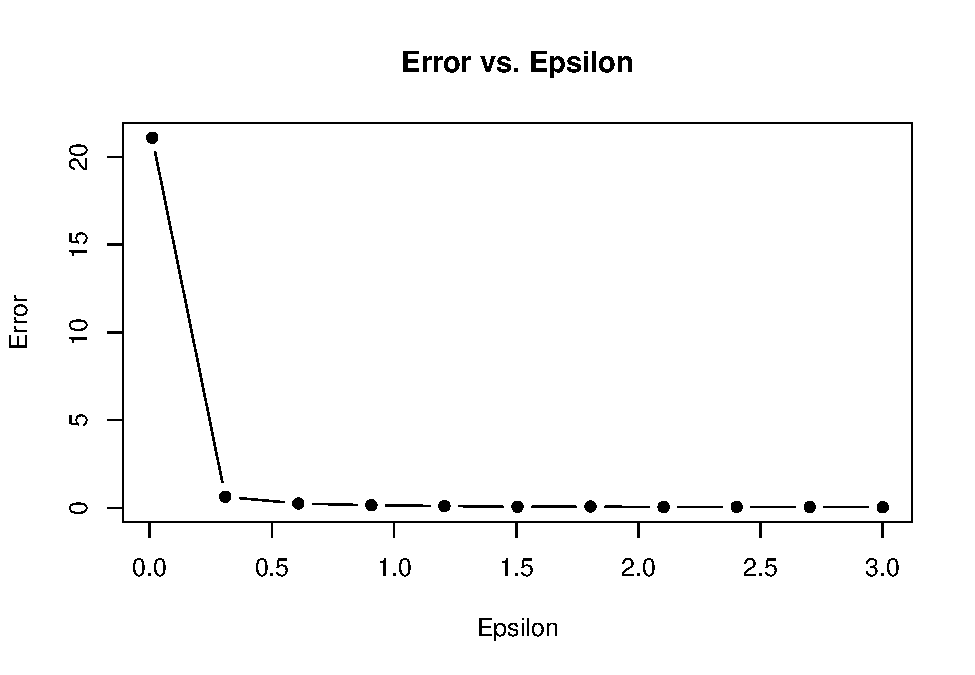
\includegraphics{DP_Second_Laboratory_files/figure-latex/unnamed-chunk-13-1.pdf}

\end{document}
